% !TEX TS-program = XeLaTeX
% use the following command:
% all document files must be coded in UTF-8
\documentclass[english]{textolivre}
% build HTML with: make4ht -e build.lua -c textolivre.cfg -x -u article "fn-in,svg,pic-align"

\journalname{Texto Livre}
\thevolume{16}
%\thenumber{1} % old template
\theyear{2023}
\receiveddate{\DTMdisplaydate{2022}{11}{22}{-1}} % YYYY MM DD
\accepteddate{\DTMdisplaydate{2022}{12}{8}{-1}}
\publisheddate{\DTMdisplaydate{2023}{1}{14}{-1}}
\corrauthor{Magdalena López Pérez}
\articledoi{10.1590/1983-3652.2023.41886}
%\articleid{NNNN} % if the article ID is not the last 5 numbers of its DOI, provide it using \articleid{} commmand 
% list of available sesscions in the journal: articles, dossier, reports, essays, reviews, interviews, editorial
\articlesessionname{dossier}
\runningauthor{López Pérez y De la Maya Retamar} 
%\editorname{Leonardo Araújo} % old template
\sectioneditorname{Hugo Heredia Ponce}
\layouteditorname{Thaís Coutinho}

\title{Reading practices in the network of trainee teachers in Primary Education}
\othertitle{Práticas literárias na rede de futuros professores do ensino primário}
% if there is a third language title, add here:
%\othertitle{Artikelvorlage zur Einreichung beim Texto Livre Journal}

\author[1]{Magdalena López Pérez~\orcid{0000-0001-6233-1719}\thanks{Email: \href{mailto:magdalenalopez@unex.es}{magdalenalopez@unex.es}}}
\author[1]{Guadalupe de la Maya Retamar~\orcid{0000-0003-4201-4024}\thanks{Email: \href{mailto:gmaya@unex.es}{gmaya@unex.es}}}
\affil[1]{Universidad de Extremadura, Facultad de Educación y Psicología, Departamento de Didáctica de las Ciencias Sociales, las Lenguas y las Literaturas, Badajoz, España.}

\addbibresource{article.bib}
% use biber instead of bibtex
% $ biber article

% used to create dummy text for the template file
\definecolor{dark-gray}{gray}{0.35} % color used to display dummy texts
\usepackage{lipsum}
\SetLipsumParListSurrounders{\colorlet{oldcolor}{.}\color{dark-gray}}{\color{oldcolor}}

% used here only to provide the XeLaTeX and BibTeX logos
\usepackage{hologo}

% if you use multirows in a table, include the multirow package
\usepackage{multirow}

% provides sidewaysfigure environment
\usepackage{rotating}

% CUSTOM EPIGRAPH - BEGIN 
%%% https://tex.stackexchange.com/questions/193178/specific-epigraph-style
\usepackage{epigraph}
\renewcommand\textflush{flushright}
\makeatletter
\newlength\epitextskip
\pretocmd{\@epitext}{\em}{}{}
\apptocmd{\@epitext}{\em}{}{}
\patchcmd{\epigraph}{\@epitext{#1}\\}{\@epitext{#1}\\[\epitextskip]}{}{}
\makeatother
\setlength\epigraphrule{0pt}
\setlength\epitextskip{0.5ex}
\setlength\epigraphwidth{.7\textwidth}
% CUSTOM EPIGRAPH - END

% LANGUAGE - BEGIN
% ARABIC
% for languages that use special fonts, you must provide the typeface that will be used
% \setotherlanguage{arabic}
% \newfontfamily\arabicfont[Script=Arabic]{Amiri}
% \newfontfamily\arabicfontsf[Script=Arabic]{Amiri}
% \newfontfamily\arabicfonttt[Script=Arabic]{Amiri}
%
% in the article, to add arabic text use: \textlang{arabic}{ ... }
%
% RUSSIAN
% for russian text we also need to define fonts with support for Cyrillic script
% \usepackage{fontspec}
% \setotherlanguage{russian}
% \newfontfamily\cyrillicfont{Times New Roman}
% \newfontfamily\cyrillicfontsf{Times New Roman}[Script=Cyrillic]
% \newfontfamily\cyrillicfonttt{Times New Roman}[Script=Cyrillic]
%
% in the text use \begin{russian} ... \end{russian}
% LANGUAGE - END

% EMOJIS - BEGIN
% to use emoticons in your manuscript
% https://stackoverflow.com/questions/190145/how-to-insert-emoticons-in-latex/57076064
% using font Symbola, which has full support
% the font may be downloaded at:
% https://dn-works.com/ufas/
% add to preamble:
% \newfontfamily\Symbola{Symbola}
% in the text use:
% {\Symbola }
% EMOJIS - END

% LABEL REFERENCE TO DESCRIPTIVE LIST - BEGIN
% reference itens in a descriptive list using their labels instead of numbers
% insert the code below in the preambule:
%\makeatletter
%\let\orgdescriptionlabel\descriptionlabel
%\renewcommand*{\descriptionlabel}[1]{%
%  \let\orglabel\label
%  \let\label\@gobble
%  \phantomsection
%  \edef\@currentlabel{#1\unskip}%
%  \let\label\orglabel
%  \orgdescriptionlabel{#1}%
%}
%\makeatother
%
% in your document, use as illustraded here:
%\begin{description}
%  \item[first\label{itm1}] this is only an example;
%  % ...  add more items
%\end{description}
% LABEL REFERENCE TO DESCRIPTIVE LIST - END


% add line numbers for submission
%\usepackage{lineno}
%\linenumbers

\begin{document}
\maketitle

\begin{polyabstract}
\begin{abstract}
The increased presence of adolescents and young people on the Internet has led to an interest in analysing their reading and multimodal practices, which sometimes involve the creation of spaces for reading socialisation in this context and the development of vernacular practices on the Internet \cite{cassany_en_linea._2012}. In this paper, we want to explore this question in greater depth, considering their reading practices on the web and the knowledge that teacher trainees in Primary Education at the University of Extremadura have about the new genres developed in this media context. For this purpose, an \textit{ad hoc} questionnaire was designed in which the students reported on their reading habits and practices. The results show a scarce knowledge of the genres mentioned and very little consolidated reading habits, which makes it necessary to carry out specific work to reinforce this habit and their knowledge of the different practices.

\keywords{Reading practices \sep Reading habits \sep Trainee teachers \sep Primary education \sep Booktubers}
\end{abstract}

\begin{portuguese}
\begin{abstract}
O aumento da presença de adolescentes e jovens na Internet levou a um interesse em analisar suas práticas de leitura e multimodais, o que às vezes envolve a criação de espaços de socialização da leitura nesse contexto e o desenvolvimento de práticas vernaculares na Internet \cite{cassany_en_linea._2012}. Neste artigo, queremos explorar essa questão com mais profundidade, considerando quais são as práticas de leitura na web e o conhecimento que os professores da escola primária em treinamento da Universidade da Extremadura têm sobre os novos gêneros desenvolvidos nesse contexto de mídia. Para esse fim, foi elaborado um questionário \textit{ad hoc} no qual os alunos relataram seus hábitos e práticas de leitura. Os resultados mostram um conhecimento escasso dos gêneros acima mencionados e hábitos de leitura muito pouco consolidados, o que torna necessário realizar um trabalho específico para reforçar esse hábito e seu conhecimento das diferentes práticas. 

\keywords{Práticas de leitura \sep Hábitos de leitura \sep Professores estagiários \sep Educação primária \sep Booktubers}
\end{abstract}
\end{portuguese}
% if there is another abstract, insert it here using the same scheme
\end{polyabstract}

\section{Introduction}\label{sec-intro}

Technological advances in recent decades have not only transformed our daily lives but have also led to numerous changes in educational processes in general, and in the process of reception and appropriation of literary culture, which has made use of the communicative and creative potential of the web \cite{paladines-paredes_videoresenas_2021a}. The participation of young people in digital environments has multiplied with the generalisation of Internet access, having reached 99.7\% of the population aged between 17 and 24 in 2021 \cite{instituto_nacional_de_estadistica_ine_encuesta_2021}. Thus, we can say that digital media have come to be considered one of the main agents of socialisation \cite{gordo_lopez_jovenes_2018}. Not surprisingly, we are facing a generation of digital natives, who have grown up after the birth of the Internet and are permanently surrounded by screens and technological artefacts \cite{cassany_en_linea._2012}. This author, citing Presnky (2001, 2004), summarises their characteristics: they are comfortable with hypertextual and multimodal documents, they multitask or do parallel processing, they are connected to the network whenever possible, they are cooperative, and they are used to immediacy and informal and playful learning.

This greater presence of adolescents and young people on the Internet has led to an interest in analysing their reading and multimodal practices, which sometimes involve the creation of spaces for reading socialisation in this context and the development of vernacular practices on the Internet \cite{cassany_en_linea._2012}. These practices are defined by this researcher as “the set of literate tasks that occur in the private and idle sphere of family and friends, which we do on our own initiative, when and how we feel like it and without following any rules or guidelines” \cite[p. 92]{cassany_en_linea._2012}\footnote{This quotation was originally in Spanish, and it has been translated into English by the authors. This has been done with all the quotations having this symbol}. On the web, young people read, but at the same time, they create, invent, comment, and share their book readings through videos, blogs, and social networks. In this way, internet has become, as \textcite{manresa_practicas_2016} point out, citing \textcite[p. 54]{leveratto_internet_2008}, a natural observatory that makes new possibilities for research on reading viable because “it offers the opportunity to analyse not only the type of reading practices that take place in virtual spaces on literary reading, but also what the reader ‘expresses’ about the literature he or she reads”.

Studies on the reading habits of children and young people show that students’ personal reading decreases as they progress through the academic years \cite{gonzalez2017habitos, valdes2018}. However, as some studies have found, the use of web 2.0 platforms is transforming the way young people share their reading experiences \cite{garcia2015leer, travancas2014juventud}. The possibilities offered by the internet and social networks to connect readers create a space for virtual interaction that consolidates a community of practice and learning \cite{paladines-paredes_canales_2020}.

Understanding the impact of the virtual environment on the reading practices of young people who use the tools provided by the Internet to generate and share content about their literary readings is of great interest for the teaching of literature. Indeed, schools cannot turn their backs on the effects of social networks on the configuration of the “empirical reader” \cite{bombini2006practicas}. Therefore, knowing the characteristics of this reader is essential to adjust school literary reader training to this new reality, both to incorporate the forms of socialisation of reading that may be of interest to the school, and to consider the training needs that arise from their actions in the virtual environment \cite{manresa_practicas_2016}.

The interactions generated on the net frequently refer to popular mass culture, hence their exclusion from school curricula \cite{torrego_gonzalez_practicas_2021}. Similarly, the development of new discursive genres, which update and expand the formats of criticism and literary tradition \cite{paladines-paredes_booktubers:_2021b} or the new emerging forms of literature \cite{abdad_ruiz_fanfiction:_2011}, such as the creation and publication of amateur literary works, are not usually considered by schools either. It is therefore necessary to analyse these practices, due to the radical change in the ways of reading and writing and the obligation we, as teachers, should train critical readers and writers on the web.

In this respect, not only have currents emerged conceptualising the processes of reading and writing from a new perspective and explaining the emergence of these new genres, but, in the last decade, research has been interested in these literary practices and in the use of platforms and networks that allow young people to have digital spaces “to convert their reading activity into a social practice mediated by technology” \cite[p. 60]{paladines-paredes_booktubers:_2021b}.  

Thus, for example, many studies have been interested in booktubers. The emergence of the booktuber phenomenon brings together teenagers who, attracted by the visual potential offered by YouTube and the ease of creating channels with their own content and free broadcasting, generate new virtual communities that discuss and analyse readings using video to share their reading experience. \textcite{ravettino_destefanis_booktubers_2015} defines booktubers as young book lovers who present and review titles on video in a virtual community of practice that includes many young people. The research has been interested, among other aspects, in identifying the main references among Spanish-speaking booktubers \cite{hernandez_ortega_nuevos_2021}, carrying out case studies on booktubers’ channels \cite{vizcaino-verdu_reading_2019, lopez-gil_promocion_2021}, the characteristics of the consumers of these channels \cite{noguera_habitos_2020}, analyse the discursive genre of video reviews \cite{paladines-paredes_videoresenas_2021a} or identify the transformations in cultural practices on literary readings introduced by the platform \cite{paladines-paredes_canales_2020}.

In booktrailers, on the other hand, as \textcite{rovira-collado_booktrailer_2017} points out, cinema and literature converge when a work of literature is presented through a medium typical of the seventh art, the trailer. Although their conception and dissemination respond to the advertising strategies of publishers, the researcher proposes their didactic exploitation and creation by students as strategies for their training and reading encouragement, as well as the analysis of some of them (2022). Once again, we are facing with a phenomenon whose study shows an increasing presence in the scientific literature, a sign of the growing interest in the socialisation of cultural behaviour among the most digitally literate sectors of the population \cite{cordon_garcia_socializacion_2023}.

Likewise, other works address literary blogs managed by teenagers as another modality of literary socialisation practices. Thus, in the study by \textcite[p.68]{manresa_practicas_2016}, the results of the analysis of five literary blogs show “the reconversion of the amateur reader into a reader who promotes and stimulates reading, as well as an expert reader who dominates the literary world and shows his or her maturity as a reader”. For their part, \textcite{sanchezgarcia_lectura_2013}, in their case study of the blogs participating in the DELIRIUM challenge, conclude that, in these blogs, the participants construct their virtual identity from reading, which they understand not only as a hobby but also as part of their lives. Furthermore, this practice transforms adolescents and shows them to the world as a network of readers capable not only of expressing their opinions, but also of generating opinions about reading.

Finally, another literary practice that is also very common is fanfiction, which refers to the “fiction of fans or ‘fanatics’ about an already created work” \cite[p.65]{martos_nunez_tunear_2006}, in which a previous source is recreated, whether literary or elaborated in different languages and media, or imaginary universes belonging to different series are crossed. The Internet has favoured its expansion by facilitating the publication of these amateur literary works and, in addition to analysing this phenomenon \cite{luna_pena_lectura_2020, quiroga_terreros_formas_2017, perez_silva_internet_2020} some teachers and researchers have made use of its didactic advantages to promote creative writing in the classroom \cite{abdad_ruiz_fanfiction:_2011, paterna_roda_fanfiction_2018}.

If we focus on the analysis of the reading profile of future teachers in general, the results of the research carried out are not flattering. \textcite[p.44]{granado_teachers_2014} states that future teachers are “not very assiduous and immature readers, frequent little variety of texts, do not place great value on books, overestimate their reading practice, make little use of libraries and make a merely instrumental use of reading”. \textcite{munita_reading_2014}, for his part, explains that the students from the University of Barcelona present a profile defined by discontinuous reading trajectories, few intertexts and reading practices mainly related to best sellers. \textcite{vera_valencia_reading_2017}, this time with students from Faculties of Education in Castilla la Mancha, confirms the lack of continuity with which future teachers read, as only 6\% of his sample can be considered frequent readers. At the University of Cadiz, the study carried out by \textcite{trigo_habitos_2020} shows that future teachers constitute a population which does not read much and whose reading corpus is made up of sagas aimed at young people or adults, current narrative works with high sales rates and some pedagogical works of an informative nature. We find somewhat different results in the study by \textcite{castillo_rodriguez_habitos_2022}, focusing on students at the University of Malaga, which shows that trainee teachers read regularly in their mother tongue, being their reading frequency ‘every day’ or ‘a few times a week’. In Extremadura, the region in which this study is contextualised, we are not aware of any study, which has analysed the mother tongue reading habits of future teachers, although there is one study dealing with those related to foreign languages \cite{de_la_maya_retamar_habitos_2021}. There is, however, one study on university students at the University of Extremadura in general \cite{perez-parejo_habitos_2019}. Among the results, the researchers highlight that more than 75\% of university students read in their free time, preferably on paper, and spend just under two hours a week on reading. The main function of reading is mainly functional, and it is almost never among the first choices as a means of leisure. 

However, as \textcite{ballester_educacion_2016} point out, research on reader profiles and reading habits does not consider, in many cases, the practices involved in reading and, often, the production of texts in digital contexts. \textcite[p. 585]{putro_profiles_2018} also argue that “the pace of development in today’s digital age has rendered much of the previous research on students' reading behaviour obsolete”. Therefore, it does not seem logical to address this profile without taking them into account: “It is essential to understand the different ways of reading, communicating, producing and appropriating texts as a basic component of any reading promotion policy, and consequently, of contemporary reading and literary training” \cite[p.154]{ballester_educacion_2016}. We are not aware of any studies that assess these practices among future primary school teachers, although we do know of some research carried out with university students. Thus, \textcite{alcocer_vazquez_practicas_2021} analyse reading practices in the digital age among university students according to their field of study: social sciences and exact sciences. The results show that the surveyed university students interact with ICT on a daily basis. Their participatory practices on the Internet related to reading are in the form of comments on social networks. However, creative production is not very widespread.

Therefore, the aim of this article is to analyse the reading profile as well as the online literary practices of future Primary Education teachers who are studying at the Faculty of Education from the University of Extremadura. In addition, we will also analyse whether there are statistically significant differences in relation to educational level and gender. To do so, we will analyse their reading habits, in a general way, to delve deeper into their reading practices on the Internet.





\section{Methodology}

The research design used is cross-sectional, descriptive, and non-correlational. The sampling carried out was not probabilistic, as the students were chosen intentionally, by convenience \cite{flyvbjerg_five_2006}.


\subsection{Participants}

The final sample of the present research was composed of 285 students ($n=285$) from the Faculty of Education and Psychology at the University of Extremadura (Spain). The participants were distributed as follows: 152 students in the first year of the Degree in Primary Education (53.5\%); 95 students in the third year of the same degree (33.3\%) and 38 students (13.2\%) in their fourth year belonging to the Itineraries of Specialisation in Foreign Languages, in Physical Education and in Audition and Language. The students from the second year of the degree were in their training period, the reason why they have not taken part in the research. As regards gender, the sample is distributed in the following way: 194 women (68.2\%) and 91 men (31.8\%). The average age of the participants is 19.88 years old.


\subsection{Instrument}
The data collection was carried out using part of the questionnaire proposed and validated by \textcite{igarza_metodologicomun_2014} to measure the reading behaviour in digital and conventional environments. As the questionnaire itself was quite long, we have considered only those questions which were pertinent for the current study, having some of them adapted. In addition, some questions of our own elaboration have been included to deepen some aspects. The final questionnaire consisted of three dimensions: 

 \begin{enumerate}
     \item Characterisation of the participating students: questions regarding the genre, age, the mother tongue and other relevant aspects were included.
     \item Reader profile: the students were asked about their interests in reading, experiences, reading frequency, preferences, and purpose, among other aspects.
     \item Transmedia scenes: we included in this dimension questions about the possible activities the students interviewed carried out when reading, about the reading practices existing today and their possible participation in reading platforms and/or social networks.
 \end{enumerate}
   


\subsection{Procedure}
Participants completed the questionnaire in Spanish during the academic year 2021/2022 in a single session, being informed of the objectives of the research and of the voluntary and anonymous nature of their participation. The questionnaire was administered online through a Google Forms link and a Qr code for the students to answer the questions in class. Before filling it, they signed their consent form.

\subsection{Statistical analysis}
Based on the data obtained from the processing of the responses provided, we have carried out a descriptive and inferential analysis to obtain answers to those aspects that we want to analyse. Given that the questionnaire had already been validated previously by its authors, we proceeded to determine the suitability of the statistical tests to be carried out. A descriptive statistical analysis was performed for all qualitative (n and \%) and quantitative ($\chi$ and SD) variables in the study. After verifying that the assumption of normality of the data was not met ($p < 0.05$), it was decided to use the non-parametric Kruskal Wallis H test and Mann-Whitney U test. For these inferential analyses, the statistical programme SPSS 23 (IBM Corp. Released 2012. IBM SPSS Statistics for Windows, Version 23. Armonk, NY: IBM Corp) was used.


\section{Results}
Once we have presented the features of the sample with the data obtained in the dimension relating to the characterisation of the participating students, we proceed to comment on the results in relation to the second dimension of our study, the reader profile.

The first question referred to their level of interest according to the kind of reading they perform that is, reading for necessity or for pleasure. The results in —\Cref{fig01}— show that most of the students read a little either for pleasure (109 students) or for necessity (103 students), followed by 93 students who read quite a lot just for need. On the contrary, the results are similar among those who read a lot (57 students read either for pleasure or for necessity) and among those who read nothing -34 students read for pleasure whereas 30 do for necessity-:

\begin{figure}[htbp]
\centering
\begin{minipage}{0.85\textwidth}
 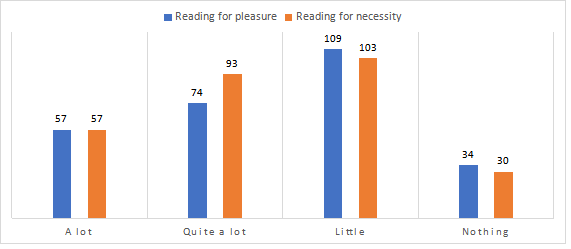
\includegraphics[width=\textwidth]{Imagem1.png}
 \caption{Level of interest according to the kind of reading performed.}
 \label{fig01}
 \source{Own elaboration.}
\end{minipage}
\end{figure}

About the second question of this dimension, ‘For what do you think the reading has been useful for you?’, 83.2\% of the respondents indicated that reading had been useful to learn, whereas another 69.6\% considered it useful for general culture. 44.1\% indicated that reading was useful to enjoy and another 43.4\%, to improve at work. It is worthy to mention that in this question students had the option of selecting multiple choices, as it can be observed in \Cref{fig02}.


\begin{figure}[htbp]
\centering
\begin{minipage}{.85\textwidth}
 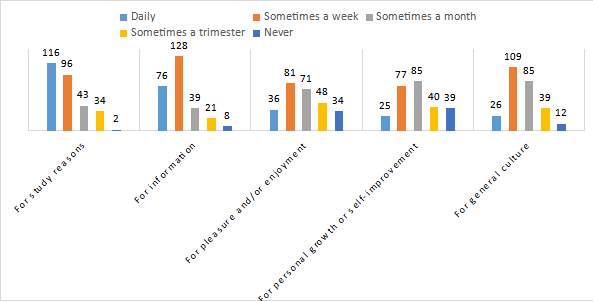
\includegraphics[width=\textwidth]{Imagem2.png}
 \caption{Reasons why you read and the frequency of each activity.}
 \label{fig02}
 \source{Own elaboration.}
\end{minipage}
\end{figure}

If we focus on the language used when reading, 283 read in Spanish but 154 students indicated having read in other languages, being English the most frequent one when reading (117 students), followed by 18 students who admit reading in Portuguese and 14 in French. As regards the reading activities that the respondents do for pleasure or for necessity, the results highlight that the reading activity that 271 students do for pleasure is to read through social nets, as \Cref{fig03} shows. This activity is followed by web pages (191 students), being the books relegated to the third position (146 students) for pleasure. If we focus on the reading activities carried out for necessity, the first one has been the email (207 students) followed by reading books (150 students), being the activity that they do least for necessity that of using social networks, just 18 students.

\begin{figure}[htbp]
\centering
\begin{minipage}{.85\textwidth}
 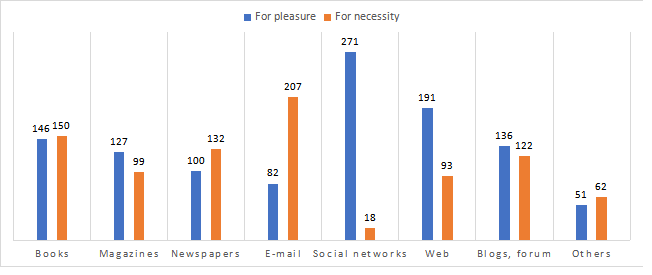
\includegraphics[width=\textwidth]{Imagem3.png}
 \caption{Reading activities that they do for pleasure or for necessity.}
 \label{fig03}
 \source{Own elaboration.}
\end{minipage}
\end{figure}

The last question of this second dimension referred to the reasons why they do not read at all, or they do not read so much. Among the answers given, the most selected one was ‘because I prefer other leisure activities’, chosen by 163 students, three less than the students who chose ‘because of lack of time’. 87 students admitted that they do not like reading and 83 of them revealed that reading makes them feel lazy.

The last dimension of our study referred to the transmedia scenes, the purpose of our research. As we have stated before, we have included questions about the possible activities that the respondents can carry out when reading, as well as about the reading practices existing today and their possible participation in reading platforms and/or social networks. 

Before commenting on the results of this dimension, we were interested in the respondents’ access to the internet and its frequency, as this could be a determinant of their responses. The results show that 284 participants have access to internet, being this access with unlimited data for the 58.2\% of the respondents. Only 3 of them (1.1\%) admitted having limited data. Also, 99.7\% indicated that they connect daily to internet and only one student answered, ‘some time a week’. Regarding the question ‘Which technological device do you use most frequently on a daily basis?’, 257 participants selected a mobile phone for personal use, followed by 166 respondents who chose a laptop or a tablet for personal use.

This question focused on whether the students do another activity while they are reading and the frequency of such an activity. The results shown in \Cref{fig04} indicate that the students never read while the television is on (153 respondents); while answering phone calls (146 respondents); while they are listening to music (135 respondents); while they are browsing the social networks (133 respondents); or while chatting (132 respondents). These results highlight the importance that they give to the act of reading as an activity for which they need to be concentrated, which is indicated in the answers given to the activity of reading every day in silence (136 respondents) or that they take notes or underline information when reading (78 respondents).

\begin{figure}[htbp]
\centering
\begin{minipage}{.85\textwidth}
 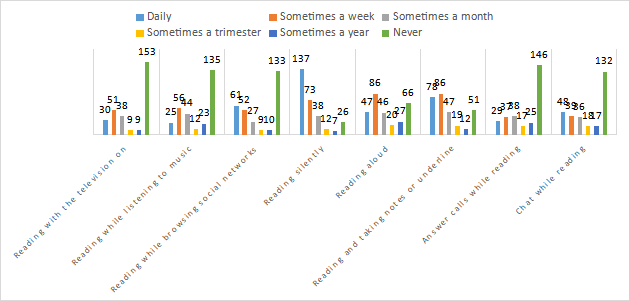
\includegraphics[width=\textwidth]{Imagem4.png}
 \caption{Activities done while reading and the frequency of each activityActivities done while reading and the frequency of each activity.}
 \label{fig04}
 \source{Own elaboration.}
\end{minipage}
\end{figure}

In the next question proposed, the students had to indicate the task that they perform related to what they have read. The results shown in \Cref{fig05} are an anticipation of the purpose of our research, as the most chosen activity was that of watching videos (212 respondents) or searching for additional information related to what they have read (180 respondents). On the contrary, what they do less is to participate in forums (15 respondents):

\begin{figure}[htbp]
\centering
\begin{minipage}{.85\textwidth}
 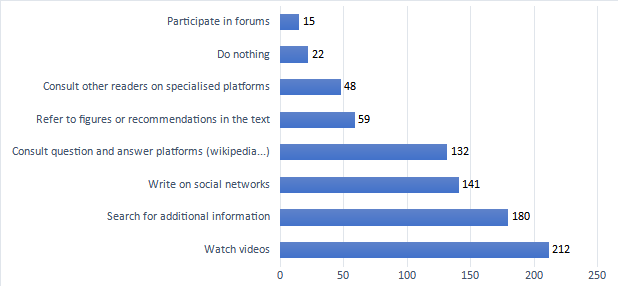
\includegraphics[width=\textwidth]{Imagem5.png}
 \caption{Which other activity do you perform related to what you have read?}
 \label{fig05}
 \source{Own elaboration.}
\end{minipage}
\end{figure}

In relation to the frequency with which they carry out the activities described above, just over a third of the participants (37.1\%) carry them out once a week, while another third (34.6\%) carry them out on a daily basis. Only 16.4\% do these activities once a month and the rest (11.4\%) do them quarterly, annually or never. In order to investigate the differences that may arise in relation to this frequency, taking the year and genre as variables, we carried out inferential analyses using non-parametric statistical tests, as the assumption of normality of the data was not met ($p<0.05$), in the case of men and first-year students. As regards gender, there are no statistically significant differences between men and women with respect to the frequency of the activities they carry out on the internet while reading. Regarding the course they are studying, the results of the Kruskal-Wallis test ($\chi^2=10.881$, $p=.004$) indicate that there are differences between the three years analysed. After comparing the means between the groups using the Mann-Whitney U test, we observe that these differences occur between the first and third year groups, in favour of the latter, i.e. the third year pupils carry out activities on the Internet more frequently in relation to their reading.

Regarding their participatory activities on the Internet linked to their readings, the topics of the texts or the author of the texts, \Cref{fig06} shows that more than half of the participants do not engage in any participation on the Internet. When participatory activities do occur, they are mostly in the form of comments on their own social networks, queries about the author or publisher on the same networks, writing emails to their contacts, following accounts on networks or blogs to keep informed about readings, authors or proposals from publishers.

\begin{figure}[htbp]
\centering
\begin{minipage}{.85\textwidth}
 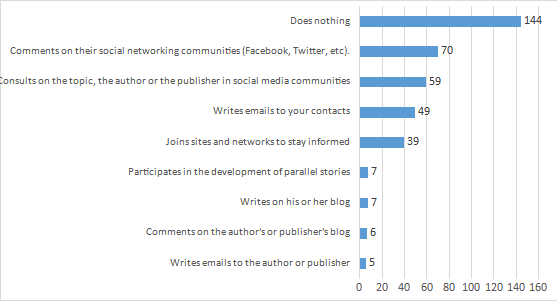
\includegraphics[width=\textwidth]{Imagem6.png}
 \caption{Participatory internet activity related to the reading, the topic or the author.}
 \label{fig06}
 \source{Own elaboration.}
\end{minipage}
\end{figure}

As far as the different literary practices on the web are concerned, literary blogs are the most popular ones among the participants, with 93 of them saying that they were familiar with one. Fanfiction is the next most popular, although in this case it is less than half of the previous case, only 48 of the participants. Booktuber and booktrailer are only residually known practices, as only 9.85\% and 4.9\% respectively say they know about them. What is most remarkable is that practically 60\% of those surveyed are not aware of any of the aforementioned practices. If we dig deeper, although some of the practices are known to them, the vast majority (94.8\%) do not claim to be followers, readers or creators of them.

Once again, we have carried out inferential analyses to determine whether there are differences by gender and/or year group in relation to their participation on the Internet, their knowledge of literary practices on the Internet and their involvement as readers or authors of these practices. Taking into consideration the gender of the participants, we found a trend contrary to the result indicated when analysing the frequency of their activities while reading, as there were no differences between men and women in this variable but now there are significant differences between them. Thus, both in the case of participatory activity on the Internet ($Z=7496.000$, $p=.018$), and in the case of knowledge of literary practices on the Internet ($Z=7396.500$, $p=.010$) and involvement as a reader or author ($Z=8287.500$, $p=.031$), men say that they participate more, know more about practices and get involved to a greater extent than women.

As regard the differences by the course, the analyses carried out using the Kruskal-Wallis test indicate that, although the average ranks of the first year students are higher than those of the other years, both in terms of their participation in Internet activity and in terms of knowledge and participation in online practices related to what they have read, there are no significant differences between them. 



\section{Discussion and conclusions}

As we have mentioned in this paper, our main objective was to establish a reading profile of the students who want to become Primary Education teachers at the Faculty of Education and Psychology from the University of Extremadura. In particular, our purpose included delving into their online literary practices, since, as \textcite{ballester_educacion_2016} pointed out, these practices were not, in many cases, considered when establishing reading profiles and habits.  

Regarding the general objective, the results have shown that reading for necessity is the one that arouses the greatest interest among future teachers, either for study reasons or for information. As for reading for pleasure, more than half of those surveyed stated that they read little or nothing, and that this is a type of reading which they mostly do on a weekly or monthly basis. Only 13\% of them read for pleasure on a daily basis. 

It is logical to think that university students have academic requirements that lead them to have to read various documents on the subjects they are studying, but it is striking that those who read for pleasure little or nothing outnumber those who read a lot or quite a lot. In other words, we are faced with future teachers who approach reading fundamentally from an instrumental perspective and this, as \textcite{alcocer_vazquez_practicas_2021} point out, represents a risk because, at the end of the compulsory relationship, the student has neither consolidated the habit of reading nor has his or her own reasons for continuing to read. In this sense, it is necessary, as \textcite{yubero_lectura_2015} point out, for the university to provide reading spaces that increase the reading behaviour of the students, on the one hand, and that support the development of reading habits, on the other. This is especially important when we talk about future teachers, because as \textcite[p.55]{granado_teachers_2014} points out, “training readers at school depends in great measure on the reading methods that the teacher models and, thus, in their own personal relationship that they hold with reading”.

In terms of the type of reading they do for necessity, books, e-mails, blogs and forums and magazines stand out. We can assume that, given that the main reasons provided for this type of reading are for studying and for looking for additional information, these are usually monographs related to the subjects they are studying in their degree courses. This fact, together with the fact that these are mainly print materials, seems to confirm the results obtained by \textcite{putro_profiles_2018} with Indonesian university students who prefer to read in print settings when the activity requires in-depth and careful thought. Email is the reading that students primarily engage in for necessity. The use of this resource as a means of communication nowadays, replacing traditional written communications and notices on bulletin boards or similar, allows them to keep abreast of issues that affect the development of their studies and the work they have to do. Finally, participation in blogs and forums for necessity can respond to the activities of exchanging opinions, questions and sharing different information, derived from online learning platforms that accompany face-to-face teaching. 

When it comes to reading for pleasure, the participants in the survey mainly opt for social networks, as it also occurs in the results obtained by \textcite{castillo_rodriguez_habitos_2022}, followed by websites, books and forums and blogs, i.e. there is a link between Web 2.0 and practices associated with voluntary reading \cite{alcocer_vazquez_practicas_2021} and its use as a means of building and strengthening social connections \cite{putro_profiles_2018}. Among the reasons given for not reading at all or not reading more frequently, the future teachers indicate, with almost the same values, a greater preference for other types of recreational activities and lack of time. Secondly, not liking reading and feeling lazy about reading are reasons given by 30\% and 29\% of respondents respectively. Again, we are talking about future teachers who do not have a consolidated reading habit and for whom reading for pleasure is not one of their frequent activities. Only half of the sample includes books in the category of reading for pleasure, 12\% of the students consider themselves non-readers and 40\%, occasional readers. These data confirm the results of other studies such as those by \textcite{munita_reading_2014}, \textcite{elche_larranaga_compleja_2019} and \textcite{trigo_habitos_2020} and highlight the lack of intrinsic motivation to read among this group, with the aggravating factor, as \textcite{felipe_morales_percepciones_2016} point out, that in a few years’ time, they will be responsible for passing on the pleasure and love of reading to their students. 

With regard to their online practices, we first investigated their possibilities of connecting to the Internet, an aspect that may be a determining factor in their practices. As in other studies and as documented by the results of the \textcite{instituto_nacional_de_estadistica_ine_encuesta_2021}, almost all of the sample had daily access to the Internet, with more than half having unrestricted access and most of them using a mobile phone, which more than half use simultaneously with a laptop or tablet. Concerning the activities they carry out related to what they read, the results show that watching videos, searching for complementary information and writing on social networks are the most frequently cited. It is clear that videos, generally those hosted on YouTube, are one of the main sources of information, as the survey carried out by \textcite{castillo_rodriguez_habitos_2022} showed, and they have become one of the activities in which young people spend the most time, with a continuous increase in the time dedicated to watching them \cite{hernandez_ortega_nuevos_2021}. This fact reinforces the need to train readers and teachers to think critically, especially in the era of post-truth and misinformation. 

As for the activities related to their reading, the subjects or the authors of their readings, which involve participation on the part of the future teachers, we find comments on their social networks as the main way of letting their reactions to what they read be known. On these same networks, the participants in this study make enquiries about the subject, the author or the publisher and become followers of pages or networks to keep themselves informed. Writing e-mails is also used as a means of sharing their reading with their contacts. However, half of the respondents do not engage in any kind of participatory activity, and only a residual percentage, around 2\%, goes further, participating in the development of parallel stories, writing their reactions in blogs or sending comments to the writer or publisher. This low level of involvement is evident when they are asked about their participation as a reader or author of these practices, an action carried out by only 5\%.

Finally, in relation to the existence of differences between the genres, we found differences in favour of women in the frequency with which they carry out activities related to their reading and in favour of men in relation to their participation on the Internet, their knowledge of literary practices on the Internet and their involvement as readers or authors of these practices. We are not aware of studies that have carried out similar analyses, but the results show that boys are more likely to take the initiative to share their experiences of what they read. With regard to differences by courses, the frequency with which first year students engage in these activities is significantly higher than those of third year students, and, although the average ranks of the first year students are higher than those of the other years, both in terms of their participation in Internet activity and in terms of knowledge and participation in online practices related to what they have read, there are no significant differences between them. This may be due to the fact that these practices are more prevalent among younger people, hence their greater participation. Some studies that have taken into consideration the course variable refer to reading habits in general, not taking into consideration online reading practices, and show that between the first and fourth year of studies the percentage of non-readers is reduced by half and the percentage of regular readers almost doubles \cite{trigo_habitos_2020}. This would be an aspect that we should look into further in order to analyse whether there is a relationship between these two practices.

The results of this study are a reflection of the changes that have occurred in the reading practices and roles of trainee teachers in the new context that is emerging in the wake of technological advances and the widespread use of the Internet. The participatory activities of future teachers in relation to what they read are still scarce, although they are beginning to be present. It is necessary to give rise to these practices in university classrooms and to initiatives that encourage the reading habits of university students in general and of future teachers in particular. As \textcite[p. 13]{alcocer_vazquez_practicas_2021} point out, knowledge of these practices, which encompass not only reading but also writing

\begin{quote}
    carries enormous potential for the constitution and promotion of reading and creative writing training programmes within universities that consider different media and platforms with the aim of rethinking what reading implies and how this act, today more than ever, involves responses, reactions and creative interactions.
\end{quote}

One of the limitations of the study is its descriptive nature, which, although necessary, only aims to bring us closer to the reality of our university classrooms. In future work, the possibility of integrating some of the aforementioned practices into the training of future teachers and subsequently evaluating their possible impact is considered.

\section{Funding}
Esta publicación de Magdalena López Pérez y Guadalupe de la Maya Retamar está cofinanciada por la Ayuda a Grupos (GR21092) de la Junta de Extremadura (Consejería de Economía, Ciencia y Agenda Digital) y FEDER “Una manera de hacer Europa”; y con el Proyecto de Innovación Docente “Adaptación del Grado de Educación Primaria a modalidad semipresencial (fase II)”, concedido por el Servicio de Orientación y Formación Docente de la Universidad de Extremadura.


\printbibliography\label{sec-bib}
% if the text is not in Portuguese, it might be necessary to use the code below instead to print the correct ABNT abbreviations [s.n.], [s.l.]
%\begin{portuguese}
%\printbibliography[title={Bibliography}]
%\end{portuguese}


%full list: conceptualization,datacuration,formalanalysis,funding,investigation,methodology,projadm,resources,software,supervision,validation,visualization,writing,review
\begin{contributors}[sec-contributors]
\authorcontribution{Magdalena López-Pérez}[conceptualization,methodology,validation,writing,review]
\authorcontribution{Guadalupe de la Maya Retamar}[methodology,formalanalysis,writing,review]
\end{contributors}



\end{document}

